\documentclass[12pt,a4paper,titlepage,headinclude,bibtotoc]{scrartcl}

%---- Allgemeine Layout Einstellungen ------------------------------------------

% Für Kopf und Fußzeilen, siehe auch KOMA-Skript Doku
\usepackage[komastyle]{scrpage2}
\pagestyle{plain}
\setheadsepline{0.5pt}[\color{black}]
\automark[section]{chapter}


%Einstellungen für Figuren- und Tabellenbeschriftungen
\setkomafont{captionlabel}{\sffamily\bfseries}
\setcapindent{0em}


%---- Weitere Pakete -----------------------------------------------------------
% Die Pakete sind alle in der TeX Live Distribution enthalten. Wichtige Adressen
% www.ctan.org, www.dante.de

% Sprachunterstützung
\usepackage[ngerman]{babel}

% Benutzung von Umlauten direkt im Text
% entweder "latin1" oder "utf8"
\usepackage[utf8]{inputenc}

% Pakete mit Mathesymbolen und zur Beseitigung von Schwächen der Mathe-Umgebung
\usepackage{latexsym,exscale,stmaryrd,amssymb,amsmath}


\usepackage[nointegrals]{wasysym}
\usepackage{eurosym}

% Anderes Literaturverzeichnisformat
%\usepackage[square,sort&compress]{natbib}
\usepackage{hyperref}
% Für Farbe
\usepackage{color}
\usepackage{graphicx}
\usepackage{wrapfig}
\usepackage{subfigure}

% Caption neben Abbildung
\usepackage{sidecap}

% Befehl für "Entspricht"-Zeichen
\newcommand{\corresponds}{\ensuremath{\mathrel{\widehat{=}}}}
% Befehl für Errorfunction
\newcommand{\erf}[1]{\text{ erf}\ensuremath{\left( #1 \right)}}

%Fußnoten zwingend auf diese Seite setzen
\interfootnotelinepenalty=1000

%Für chemische Formeln (von www.dante.de)
%% Anpassung an LaTeX(2e) von Bernd Raichle
\makeatletter
\DeclareRobustCommand{\chemical}[1]{%
  {\(\m@th
   \edef\resetfontdimens{\noexpand\)%
       \fontdimen16\textfont2=\the\fontdimen16\textfont2
       \fontdimen17\textfont2=\the\fontdimen17\textfont2\relax}%
   \fontdimen16\textfont2=2.7pt \fontdimen17\textfont2=2.7pt
   \mathrm{#1}%
   \resetfontdimens}}
\makeatother

%Honecker-Kasten mit $$\shadowbox{$xxxx$}$$
\usepackage{fancybox}

%SI-Package
\usepackage{siunitx}

%keine Einrückung, wenn Latex doppelte Leerzeile
\parindent0pt

%Bibliography \bibliography{literatur} und \cite{gerthsen}
%\usepackage{cite}
\usepackage{babelbib}
\selectbiblanguage{ngerman}

\begin{document}

\begin{titlepage}
\centering
%\textsc{\Large Praktikum zur Einführung in die physikalische Chemie,\\[1.5ex] Universität Göttingen}

\vspace*{3cm}

\rule{\textwidth}{1pt}\\[0.5cm]
{\huge \bfseries
  V1 :Interferenz\\[1.5ex]
  und Wellenlängenmessung}\\[0.5cm]
\rule{\textwidth}{1pt}

\vspace*{3cm}


\begin{Large}
\begin{tabular}{ll}
Durchführende: &  Alea Tokita, Julia Stachowiak\\
Assistentin: & Annemarie Kehl\\
 Versuchsdatum: & 09.11.2015\\
 Datum der Abgabe: & 16.11.2015\\
\end{tabular}
\end{Large}

\vspace*{2.5cm}

\begin{Large}
\fbox{
  \begin{minipage}[t][3.5cm][t]{6cm} 
   Werte:
  \end{minipage}
}
\end{Large}

\end{titlepage}

\tableofcontents

\newpage


%\textbf{Interferenz und Wellenlängenmessung am 9.11.2015} \\

%Name: Julia Stachowiak \\
%Versuchspartner: Alea Tokita \\
%Assistentin: \\ \\

\section{Theoretische Grundlagen}
Gegeben sind zwei Siebgitter, eines davon mit bekannter und eines mit unbekannter Gitterkonstante. Nacheinander werden sie mit einem Laserstrahl durchleuchtet und das entstehende Interferenzmuster ausgewertet. Ziel des Versuches ist es, daran die Wellenlänge des Lasers und anschließend die unbekannte Gitterkonstante berechnen zu können.

\subsection{Elektromagnetische Wellen}
%\begin{flushleft}
Licht ist elektromagnetische Strahlung, die aus einzelnen Transversalwellen besteht. Diese harmonischen Wellen bewegen sich mit der Lichtgeschwindigkeit $c= 299 792,458 \frac{km}{s}$ durch den Raum. Sie können durch folgende Sinusfunktion in Abhängigkeit des Ortes $x$ und der Zeit $t$ beschrieben werden:
\\
\par %= Leerzeile
$f(x,t)= A\sin(kx-wt)$
\\
\par

Die Wellenzahl $k$ mit $k=\frac{2\pi}{\lambda}$ beschreibt hierbei den Zusammenhang zwischen der Wellenlänge und der Frequenz. \\
Die Relation zu der Periodendauer $T$ gibt die Kreisfrequenz $\omega =\frac{2\pi}{T} $ an.  

%können mit folgender Sinusfunktion in Abhängigkeit zum Ort x beschrieben werden, wobei $\lambda$ die Wellenlänge beschreibt:
%\\
%$f(x)=\sin \frac{2\pi}{\lambda}x $
%\\
%Der Zusammenhang zwischen der Wellenlänge $\lambda$ und deren Frequenz wird mit der Wellenzahl k beschrieben:
%\\
%$k=\frac{2\pi}{\lambda}$

%\end{flushleft} 





%Die Wellenzahl k kann durch folgende Gleichung beschrieben werden:
%\\
 %\centering
%$k= \frac{2\pi}{\lambda}$

\subsection{Phasengeschwindigkeit und Gangunterschied}
Die Ausbreitungsgeschwindigkeit $c$, mit der sich eine Phase einer Welle (der augenblickeliche Zustand, z.B. ein Minimum) im Raum fortbewegt, wird als Phasengeschwindigkeit $v$ in Abhängigkeit zu der Frequenz $v=\frac{1}{T}$ und der Wellenlänge $\lambda$ beschrieben:\\
\par
$\vec{v}_p = v\lambda$
\\
\par

Die Phasengeschwindigkeit wird durch folgende Grafik verdeutlicht:

\begin{figure} [h]
\begin{center}
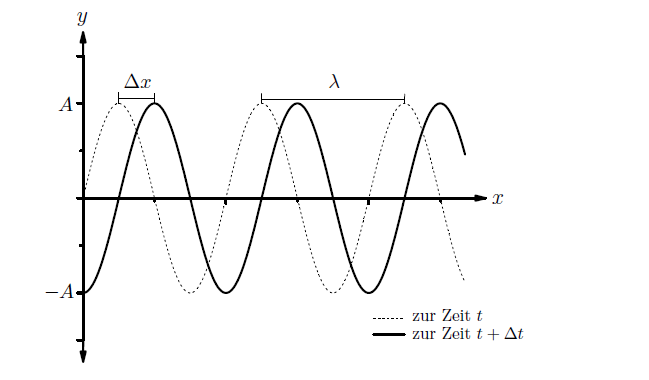
\includegraphics[scale=0.75]{Phasengeschwindigkeit2.png} \end{center}
\caption{Phasengeschwindigkeit und Gangunterschied}
\end{figure}
%Achtung: hier Phasengeschwindigkeit als c

Werden zwei Wellen mit gleicher Phasengeschwindigkeit zeitlich verzögert ausgesandt, so ergibt sich eine Wegdifferenz $\Delta x$, der sogenannte Gangunterschied $\delta$. 

\subsection{Interferenz}
Überlagern sich zwei oder mehr Wellen, so führt dies zu einer Amplitudenänderung. Die Wellen verschmelzen zu einer neuen Welle mit größerer oder kleinerer Amplitude, je nachdem, ob gleiche oder unterschiedliche Phasen aufeinandertreffen. Diese Erscheinung nennt man Interferenz. Treffen Maxima oder Minima aufeinander, so wird die Amplitude verstärkt (konstruktive Interferenz); trifft Maximum auf Minium so löschen sich die Wellen gegenseitig aus (destruktive Interferenz). 
Eine konstruktive Interferenz zweier Wellen ist demnach nur möglich, wenn der Gangunterschied ebendieser ganzzahliges Vielfaches der Wellenlänge ist:\\
\par
$\delta=n \lambda$ mit $n = 0,1,2...$
\\
\par

Ist $\delta$ jedoch ein ungradzahliges Vielfaches der halben Wellenlänge, so tritt destruktive Interferenz auf. \\
\par
$\delta = \frac{(2n+1)\lambda}{2}$ mit $n=0,1,2...$
\\
\par


\subsection{Streuung und Beugung}
Trifft eine Welle auf ein Hindernis, so verändert sie ihren geometrisch vorgeschriebenen Weg, dh. sie wird gestreut. %Der Begriff Streuung ist ein Sammelbegriff für viele physikalische Phänomene wie Reflexion, Brechung, Beugung etc., bei denen die Welle außerdem ihre Phase und Wellenlänge $\lambda$ verändern kann. 
Trifft ein Wellenzug senkrecht auf ein Gitter mit der Gitterkonstante $d$, so werden seine verschiedenen Wellen an benachbarten Gitterstäben unter dem Beugungswinkel $\beta_n$ gebeugt. Konstruktive Interferenz ergibt sich nur, wenn der Gangunterschied dieser Wellen Formel NR. [NUMMERIERUNG angeben!!!] entspricht, dh. ein ganzzahliges Vielfaches beträgt.

[Grafik aus Skript zum Gangunterschied einfügen]

Bildet man das entstehende Muster auf einem Schirm ab, so entsteht ein Beugungsbild der Wellen mit je ganzzahligem Gangunterschied. [.........]

\section{Experimentelles}

\subsection{Versuchsaufbau}

\subsubsection{Skizze der Apparatur}
\begin{figure} [h]
\begin{center}
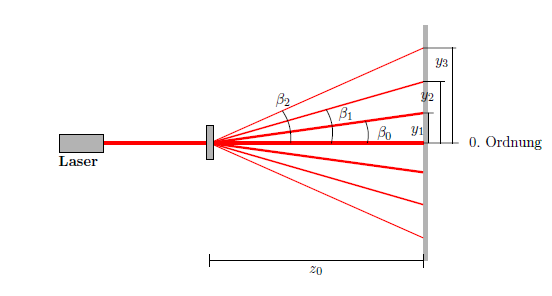
\includegraphics[scale=1]{Versuchsaufbau.png} \end{center}
\caption{Versuchsaufbau}
\end{figure}

Zunächst wird der Versuch wie auf der Skizze beschrieben aufgebaut.
Ein Laser strahlt auf ein Siebgitter, wodurch auf einem sich dahinter befindenden, an ein Holzrahmen befestigtes, Millimeterpapier ein Interferenzmuster entsteht. Anschließend wird das Siebgitter durch ein anderes Siebgitter, nun unbekannter Gitterkonstante, ersetzt.


\subsection{Durchführung}
Die entstehenden Beugungsmuster werden auf das Papier übertragen. Dabei werden jeweils die drei Punkte  oberhalb und unterhalb des nullten Beugunsmaximum übertragen.
Nach Übertragung der Punkte werden die Millitmeterpapiere von dem Holzrahmen genommen und die Abstände $y_{y},y_{2},y_{3}$ der Punkte oberhalb des nullten Maximum zu diesem und die Abstände $y_{-1},y_{-2},y_{-3}$ unterhalb des nullten Maximum zu diesem gemessen. Außerdem wird der Abstand $z_{o}$ vom Laser zum Holzrahmen gemessen.


\section{Messwerte}


Abstand Laser- Holzrahmen: 70 cm


\begin{table} [h]
\centering
\begin{large}

\end{large}
\begin{tabular}{|p{4 cm}||p{4 cm}|p{4 cm}|}
        \hline
          Abstand  & Gitter 1  & Gitter 2 \\
          in mm & d=50,1$\mu$m & d unbekannt\\
         
         
         \hline 
         $y_3 $& 28 & 16 \\
         \hline
         $y_2 $& 19 & 11\\
         \hline
         $y_{1} $& 9,0 & 6 \\
         \hline
         $y_{-1}$& 9,0 & 5 \\
         \hline
         $y_{-2}$& 18 & 11 \\
         \hline             
         $y_{-3}$& 28 & 17 \\
         \hline
\end{tabular}
\end{table}



\section{Auswertung}

Ja aber am Schluss ist es explodiert!

\section{Fehlerrechnung}
\subsection{Fehlerfortpflanzung}
Im Versuch entstehen Fehler, sowohl durch die Messungen mit dem Zollstock als auch bei der Übertragung und Ausmessen der Werte auf dem Millimeterpapier. Messungenauigkeiten beim Messen mit dem Zollstock entstehen dadurch, dass es schwierig ist, den Zollstock exakt so anzulegen, dass die kürzeste Strecke zwischen Holzrahmen und Laser gemessen wird, auch ist die Skalierung nur auf einen Millimeter genau gegeben. Wir gehen daher von folgendem Fehler aus: $\Delta_{Zollstock}={2} \cdot{10^{-2}}m$. Die Messungenauigkeiten bezüglich des Millimeterpapiers entstehen durch ungenaue Übertragung, etwa sind die Laserpunkte eher in Tropfenform, sodass der Mittelpunkt nicht exakt bestimmt werden kann, des weiteren ist die Messung der Abstände nur auf Millimeter genau. $\Delta_{Millimeterpapier}={2} \cdot {10^{-3}}$

    

\subsection{Diskussion systematischer Fehler}



\subsection{Vergleich mit Literaturwerten}

\section{Literaturverzeichnis}

%\textbf{Interferenz und Wellenlängenmessung am 9.11.2015} \\

%Name: Julia Stachowiak \\
%Versuchspartner: Alea Tokita \\
%Assistentin: \\ \\



%\begin{table}
%\centering
%\begin{large}

%\end{large}
%\begin{tabular}{|p{4 cm}||p{4 cm}|p{4 cm}|}
  %      \hline
   %       Abstand  & Gitter 1  & Gitter 2 \\
    %      \textit{in cm} & & \\
         
         
     %    \hline 
      %   $y_3 $& & \\
      %   \hline
      %   $y_2 $& & \\
      %   \hline
      %   $y_{1} $& & \\
         
      %   \hline
      %   $y_{-1}$& & \\
      %   \hline
      %   $y_{-2}$& & \\
       %  \hline             
       %  $y_{-3}$& & \\
     %    \hline
%\end{tabular}
%\end{table}




\end{document}


